\documentclass{hcmut-report}
\usepackage{codespace}
\usepackage{graphicx}
\usepackage{hyperref}
\usepackage{float}

\title{Lab 1: LED Animations}
\coursename{Microcontroller}
\reporttype{Lab Report}
\stuname{Âu Lê Quang Trí - 2453300} 

\begin{document}
\coverpage

\tableofcontents
\newpage

\section{Exercise 1}
\subsection*{Report 1: Schematic}
The Proteus schematic for this exercise is shown below. 

\begin{figure}[H]
    \centering
    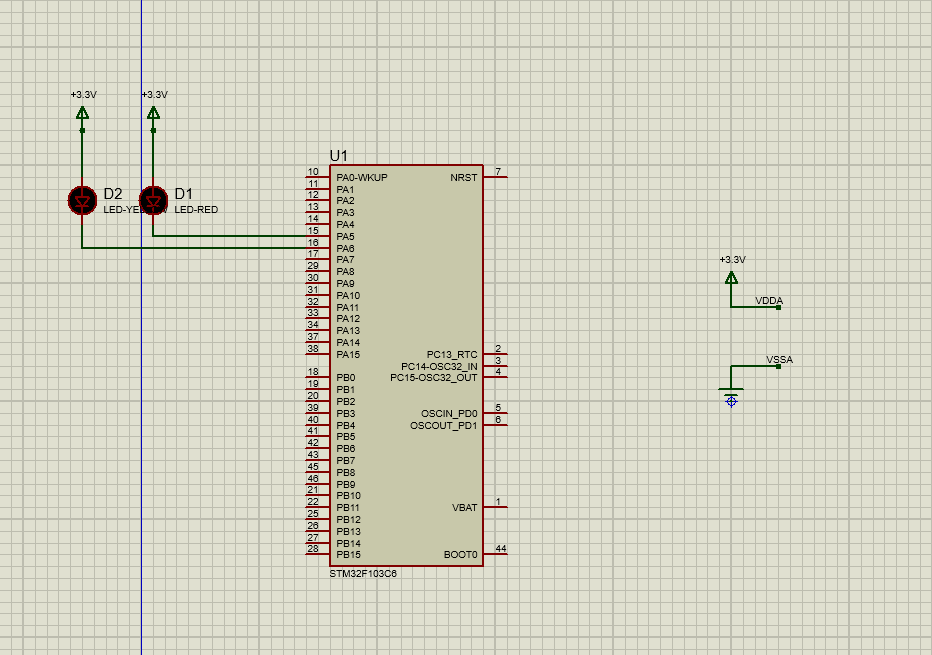
\includegraphics[width=0.8\textwidth]{images/ex1.png}
    \caption{\url{https://github.com/aulequangtri/microprocessor_lab}}
\end{figure}

\subsection*{Report 2: Source Code}
The source code inside the \texttt{while(1)} loop to switch the states of the RED and YELLOW LEDs every 2 seconds:

\begin{code}{c}
  while (1)
  {
      HAL_GPIO_TogglePin(LED_RED_GPIO_Port, LED_RED_Pin);
      HAL_GPIO_TogglePin(LED_YELLOW_GPIO_Port, LED_YELLOW_Pin);
      HAL_Delay(1000);
  }
\end{code}

\section{Exercise 2}
\subsection*{Report 1: Schematic}
The Proteus schematic for the 3-LED traffic light system is shown below.

\begin{figure}[H]
    \centering
    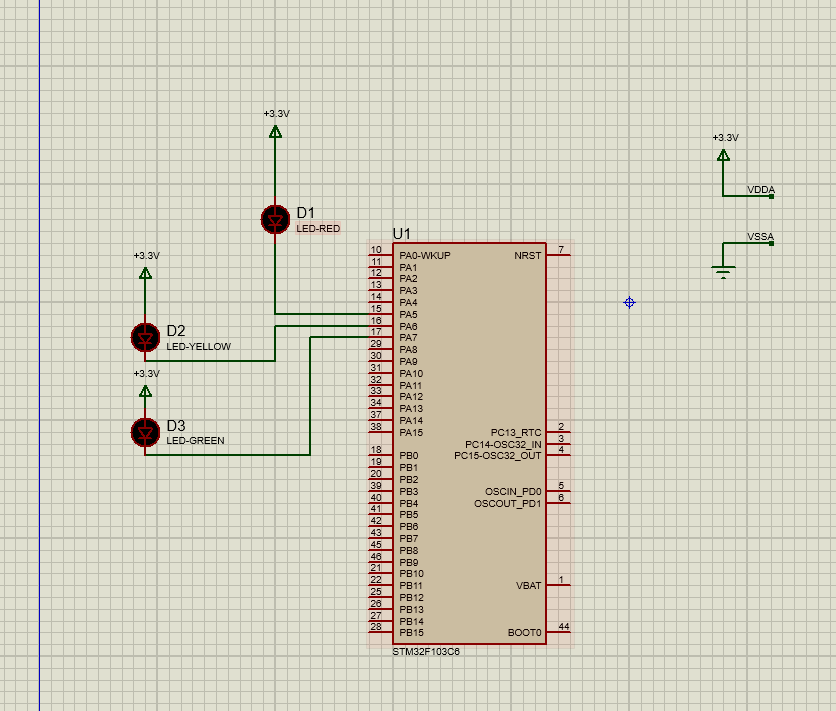
\includegraphics[width=0.8\textwidth]{images/2.png}
    \caption{Schematic for Exercise 2 (Traffic Light)}
\end{figure}

\subsection*{Report 2: Source Code}
The source code inside the \texttt{while(1)} loop simulating the traffic light cycle:

\begin{code}{c}
  while (1)
  {
      HAL_GPIO_WritePin(LED_RED_GPIO_Port, LED_RED_Pin, RESET);
      HAL_GPIO_WritePin(LED_YELLOW_GPIO_Port, LED_YELLOW_Pin, SET);
      HAL_GPIO_WritePin(LED_GREEN_GPIO_Port, LED_GREEN_Pin, SET);
      HAL_Delay(5000);

      HAL_GPIO_WritePin(LED_RED_GPIO_Port, LED_RED_Pin, SET);
      HAL_GPIO_WritePin(LED_YELLOW_GPIO_Port, LED_YELLOW_Pin, SET);
      HAL_GPIO_WritePin(LED_GREEN_GPIO_Port, LED_GREEN_Pin, RESET);
      HAL_Delay(3000);

      HAL_GPIO_WritePin(LED_RED_GPIO_Port, LED_RED_Pin, SET);
      HAL_GPIO_WritePin(LED_YELLOW_GPIO_Port, LED_YELLOW_Pin, RESET);
      HAL_GPIO_WritePin(LED_GREEN_GPIO_Port, LED_GREEN_Pin, SET);
      HAL_Delay(2000);
  }
\end{code}

\section{Exercise 4}
\subsection*{Report 1: Schematic}
The schematic for the 7-segment display integration.

\begin{figure}[H]
    \centering
    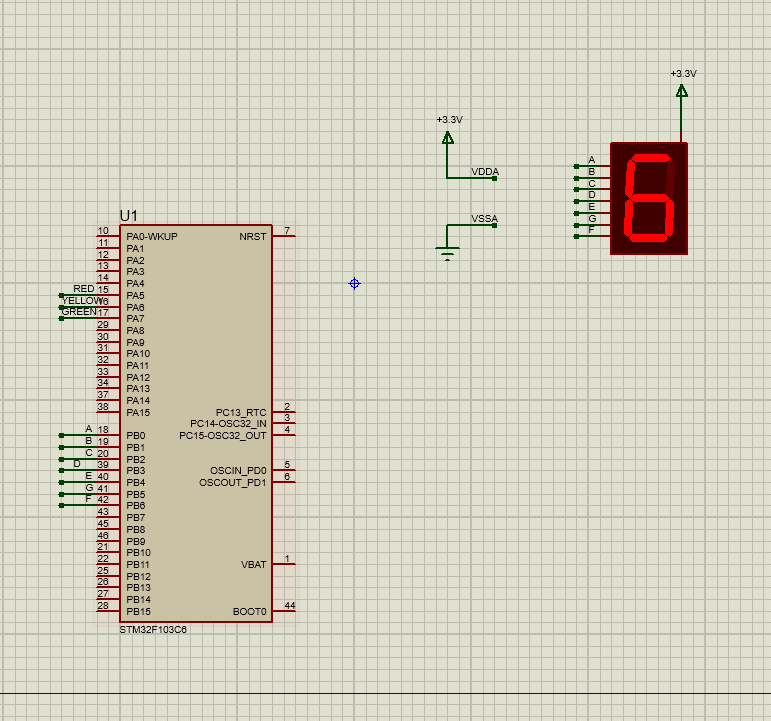
\includegraphics[width=0.8\textwidth]{images/ex4.png}
    \caption{Schematic for Exercise 4 (7-Segment LED)}
\end{figure}

\subsection*{Report 2: Source Code for display7SEG function}
The function \texttt{display7SEG(int num)} is implemented as follows:

\begin{code}{c}
void display7SEG(int num) {
      /* Turn off all segments first */
      HAL_GPIO_WritePin(LED_A_GPIO_Port, LED_A_Pin, GPIO_PIN_SET);
      HAL_GPIO_WritePin(LED_B_GPIO_Port, LED_B_Pin, GPIO_PIN_SET);
      HAL_GPIO_WritePin(LED_C_GPIO_Port, LED_C_Pin, GPIO_PIN_SET);
      HAL_GPIO_WritePin(LED_D_GPIO_Port, LED_D_Pin, GPIO_PIN_SET);
      HAL_GPIO_WritePin(LED_E_GPIO_Port, LED_E_Pin, GPIO_PIN_SET);
      HAL_GPIO_WritePin(LED_F_GPIO_Port, LED_F_Pin, GPIO_PIN_SET);
      HAL_GPIO_WritePin(LED_G_GPIO_Port, LED_G_Pin, GPIO_PIN_SET);

      /* Turn on required segments based on the number */
      switch (num) {
          case 0:
              HAL_GPIO_WritePin(LED_A_GPIO_Port, LED_A_Pin, GPIO_PIN_RESET);
              HAL_GPIO_WritePin(LED_B_GPIO_Port, LED_B_Pin, GPIO_PIN_RESET);
              HAL_GPIO_WritePin(LED_C_GPIO_Port, LED_C_Pin, GPIO_PIN_RESET);
              HAL_GPIO_WritePin(LED_D_GPIO_Port, LED_D_Pin, GPIO_PIN_RESET);
              HAL_GPIO_WritePin(LED_E_GPIO_Port, LED_E_Pin, GPIO_PIN_RESET);
              HAL_GPIO_WritePin(LED_F_GPIO_Port, LED_F_Pin, GPIO_PIN_RESET);
              break;
          case 1:
              HAL_GPIO_WritePin(LED_B_GPIO_Port, LED_B_Pin, GPIO_PIN_RESET);
              HAL_GPIO_WritePin(LED_C_GPIO_Port, LED_C_Pin, GPIO_PIN_RESET);
              break;
          case 2:
              HAL_GPIO_WritePin(LED_A_GPIO_Port, LED_A_Pin, GPIO_PIN_RESET);
              HAL_GPIO_WritePin(LED_B_GPIO_Port, LED_B_Pin, GPIO_PIN_RESET);
              HAL_GPIO_WritePin(LED_D_GPIO_Port, LED_D_Pin, GPIO_PIN_RESET);
              HAL_GPIO_WritePin(LED_E_GPIO_Port, LED_E_Pin, GPIO_PIN_RESET);
              HAL_GPIO_WritePin(LED_G_GPIO_Port, LED_G_Pin, GPIO_PIN_RESET);
              break;
          case 3:
              HAL_GPIO_WritePin(LED_A_GPIO_Port, LED_A_Pin, GPIO_PIN_RESET);
              HAL_GPIO_WritePin(LED_B_GPIO_Port, LED_B_Pin, GPIO_PIN_RESET);
              HAL_GPIO_WritePin(LED_C_GPIO_Port, LED_C_Pin, GPIO_PIN_RESET);
              HAL_GPIO_WritePin(LED_D_GPIO_Port, LED_D_Pin, GPIO_PIN_RESET);
              HAL_GPIO_WritePin(LED_G_GPIO_Port, LED_G_Pin, GPIO_PIN_RESET);
              break;
          case 4:
              HAL_GPIO_WritePin(LED_B_GPIO_Port, LED_B_Pin, GPIO_PIN_RESET);
              HAL_GPIO_WritePin(LED_C_GPIO_Port, LED_C_Pin, GPIO_PIN_RESET);
              HAL_GPIO_WritePin(LED_F_GPIO_Port, LED_F_Pin, GPIO_PIN_RESET);
              HAL_GPIO_WritePin(LED_G_GPIO_Port, LED_G_Pin, GPIO_PIN_RESET);
              break;
          case 5:
              HAL_GPIO_WritePin(LED_A_GPIO_Port, LED_A_Pin, GPIO_PIN_RESET);
              HAL_GPIO_WritePin(LED_C_GPIO_Port, LED_C_Pin, GPIO_PIN_RESET);
              HAL_GPIO_WritePin(LED_D_GPIO_Port, LED_D_Pin, GPIO_PIN_RESET);
              HAL_GPIO_WritePin(LED_F_GPIO_Port, LED_F_Pin, GPIO_PIN_RESET);
              HAL_GPIO_WritePin(LED_G_GPIO_Port, LED_G_Pin, GPIO_PIN_RESET);
              break;
          case 6:
              HAL_GPIO_WritePin(LED_A_GPIO_Port, LED_A_Pin, GPIO_PIN_RESET);
              HAL_GPIO_WritePin(LED_C_GPIO_Port, LED_C_Pin, GPIO_PIN_RESET);
              HAL_GPIO_WritePin(LED_D_GPIO_Port, LED_D_Pin, GPIO_PIN_RESET);
              HAL_GPIO_WritePin(LED_E_GPIO_Port, LED_E_Pin, GPIO_PIN_RESET);
              HAL_GPIO_WritePin(LED_F_GPIO_Port, LED_F_Pin, GPIO_PIN_RESET);
              HAL_GPIO_WritePin(LED_G_GPIO_Port, LED_G_Pin, GPIO_PIN_RESET);
              break;
          case 7:
              HAL_GPIO_WritePin(LED_A_GPIO_Port, LED_A_Pin, GPIO_PIN_RESET);
              HAL_GPIO_WritePin(LED_B_GPIO_Port, LED_B_Pin, GPIO_PIN_RESET);
              HAL_GPIO_WritePin(LED_C_GPIO_Port, LED_C_Pin, GPIO_PIN_RESET);
              break;
          case 8:
              HAL_GPIO_WritePin(LED_A_GPIO_Port, LED_A_Pin, GPIO_PIN_RESET);
              HAL_GPIO_WritePin(LED_B_GPIO_Port, LED_B_Pin, GPIO_PIN_RESET);
              HAL_GPIO_WritePin(LED_C_GPIO_Port, LED_C_Pin, GPIO_PIN_RESET);
              HAL_GPIO_WritePin(LED_D_GPIO_Port, LED_D_Pin, GPIO_PIN_RESET);
              HAL_GPIO_WritePin(LED_E_GPIO_Port, LED_E_Pin, GPIO_PIN_RESET);
              HAL_GPIO_WritePin(LED_F_GPIO_Port, LED_F_Pin, GPIO_PIN_RESET);
              HAL_GPIO_WritePin(LED_G_GPIO_Port, LED_G_Pin, GPIO_PIN_RESET);
              break;
          case 9:
              HAL_GPIO_WritePin(LED_A_GPIO_Port, LED_A_Pin, GPIO_PIN_RESET);
              HAL_GPIO_WritePin(LED_B_GPIO_Port, LED_B_Pin, GPIO_PIN_RESET);
              HAL_GPIO_WritePin(LED_C_GPIO_Port, LED_C_Pin, GPIO_PIN_RESET);
              HAL_GPIO_WritePin(LED_D_GPIO_Port, LED_D_Pin, GPIO_PIN_RESET);
              HAL_GPIO_WritePin(LED_F_GPIO_Port, LED_F_Pin, GPIO_PIN_RESET);
              HAL_GPIO_WritePin(LED_G_GPIO_Port, LED_G_Pin, GPIO_PIN_RESET);
              break;
      }
}
\end{code}

\section{Exercise 5}
\subsection*{Report 1: Schematic}
\begin{figure}[H]
    \centering
    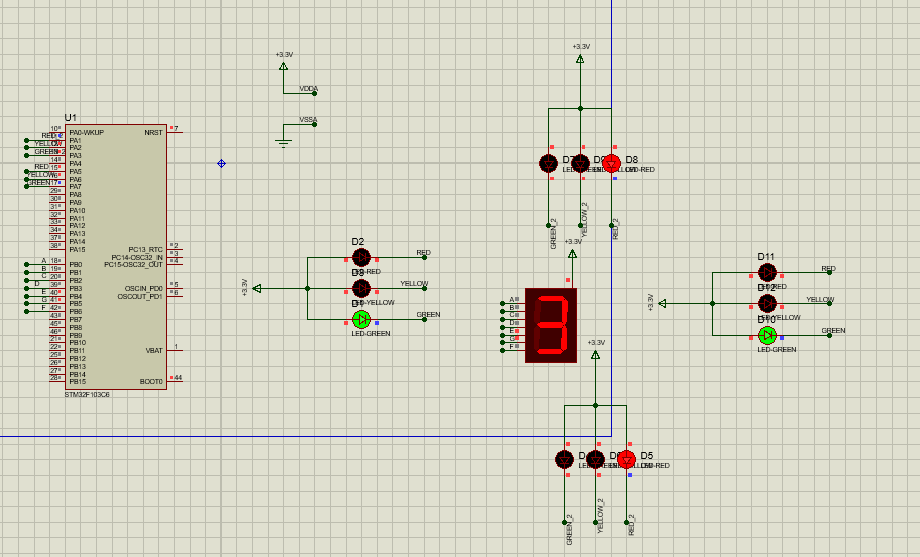
\includegraphics[width=0.8\textwidth]{images/ex5.png}
    \caption{Schematic for Exercise 5 (4-Way Traffic Light + 7SEG)}
\end{figure}

\subsection*{Report 2: Source Code}
The code snippet inside the infinite loop for the 4-way traffic light integrated with a 7-segment countdown:

\begin{code}{c}
  while (1)
  {
      display7SEG(countdown);

      HAL_GPIO_WritePin(RED_GPIO_Port, RED_Pin, GPIO_PIN_SET);
      HAL_GPIO_WritePin(YELLOW_GPIO_Port, YELLOW_Pin, GPIO_PIN_SET);
      HAL_GPIO_WritePin(GREEN_GPIO_Port, GREEN_Pin, GPIO_PIN_SET);

      HAL_GPIO_WritePin(RED_2_GPIO_Port, RED_2_Pin, GPIO_PIN_SET);
      HAL_GPIO_WritePin(YELLOW_2_GPIO_Port, YELLOW_2_Pin, GPIO_PIN_SET);
      HAL_GPIO_WritePin(GREEN_2_GPIO_Port, GREEN_2_Pin, GPIO_PIN_SET);

      if (state == 0) {
          HAL_GPIO_WritePin(RED_GPIO_Port, RED_Pin, GPIO_PIN_RESET);
          HAL_GPIO_WritePin(GREEN_2_GPIO_Port, GREEN_2_Pin, GPIO_PIN_RESET);

          countdown--;
          if (countdown <= 0) {
              state = 1;
              countdown = 2; 
          }
      }
      else if (state == 1) {
          HAL_GPIO_WritePin(RED_GPIO_Port, RED_Pin, GPIO_PIN_RESET);
          HAL_GPIO_WritePin(YELLOW_2_GPIO_Port, YELLOW_2_Pin, GPIO_PIN_RESET);

          countdown--;
          if (countdown <= 0) {
              state = 2;
              countdown = 3; 
          }
      }
      else if (state == 2) {
          HAL_GPIO_WritePin(GREEN_GPIO_Port, GREEN_Pin, GPIO_PIN_RESET);
          HAL_GPIO_WritePin(RED_2_GPIO_Port, RED_2_Pin, GPIO_PIN_RESET);

          countdown--;
          if (countdown <= 0) {
              state = 3;
              countdown = 2; 
          }
      }
      else if (state == 3) {
          HAL_GPIO_WritePin(YELLOW_GPIO_Port, YELLOW_Pin, GPIO_PIN_RESET);
          HAL_GPIO_WritePin(RED_2_GPIO_Port, RED_2_Pin, GPIO_PIN_RESET);

          countdown--;
          if (countdown <= 0) {
              state = 0;
              countdown = 3; 
          }
      }

      HAL_Delay(1000); 
  }
\end{code}

\section{Exercise 6}
\subsection*{Report 1: Schematic}
The Proteus schematic for the analog clock using 12 LEDs.

\begin{figure}[H]
    \centering
    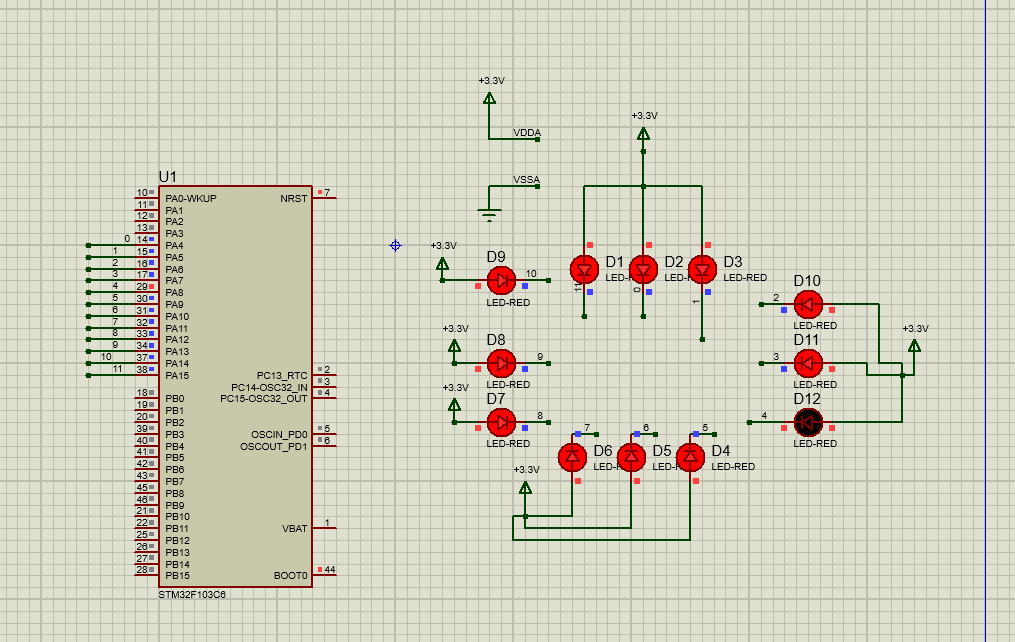
\includegraphics[width=0.8\textwidth]{images/ex6.png}
    \caption{Schematic for Exercise 6 (Analog Clock)}
\end{figure}

\subsection*{Report 2: Source Code}
The testing program turning every LED in a sequence:

\begin{code}{c}
  while (1)
  {
      HAL_GPIO_WritePin(GPIOA, clock_pins[current_led], GPIO_PIN_SET);

      current_led++;

      if (current_led >= 12) {
          HAL_Delay(1000); 

          for (int i = 0; i < 12; i++) {
              HAL_GPIO_WritePin(GPIOA, clock_pins[i], GPIO_PIN_RESET);
          }
          current_led = 0; 
      }

      HAL_Delay(500);
  }
\end{code}

\section{Exercise 7 to 10}
The following schematic is used for the analog clock exercises (7 to 10):

\begin{figure}[H]
    \centering
    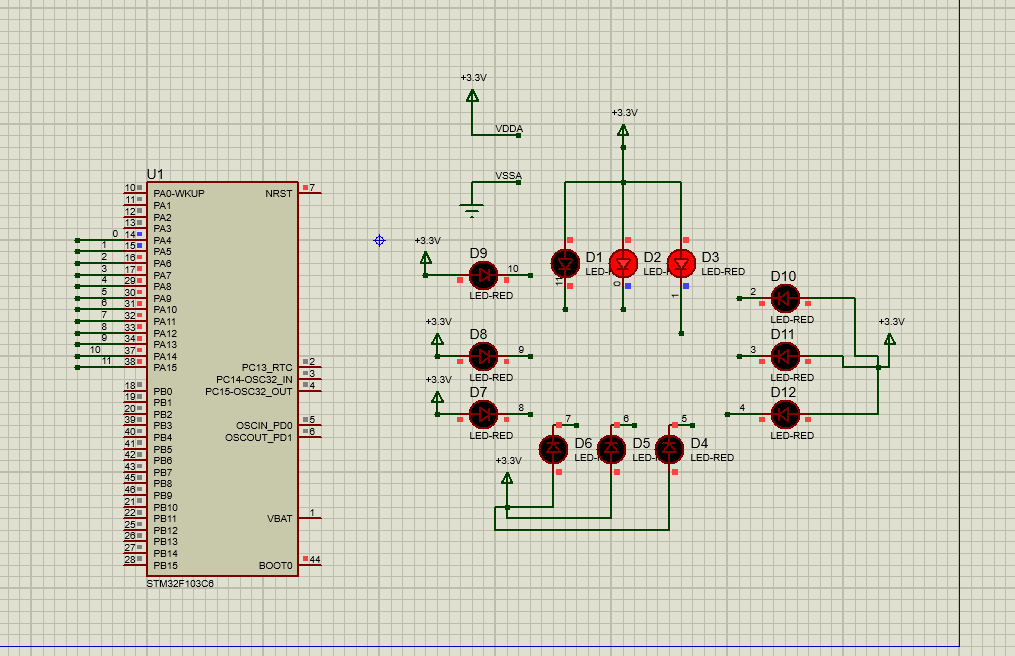
\includegraphics[width=0.8\textwidth]{images/7_to_10.png}
    \caption{Schematic for Exercises 7-10 (Analog Clock Functions)}
\end{figure}

\subsection*{Exercise 7: clearAllClock()}
\begin{code}{c}
void clearAllClock(void) {
    uint16_t all_clock_pins = GPIO_PIN_4 | GPIO_PIN_5 | GPIO_PIN_6 | GPIO_PIN_7 |
                              GPIO_PIN_8 | GPIO_PIN_9 | GPIO_PIN_10 | GPIO_PIN_11 |
                              GPIO_PIN_12 | GPIO_PIN_13 | GPIO_PIN_14 | GPIO_PIN_15;

    HAL_GPIO_WritePin(GPIOA, all_clock_pins, LED_OFF);
}
\end{code}

\subsection*{Exercise 8: setNumberOnClock(int num)}
\begin{code}{c}
void setNumberOnClock(int num) {
    if (num >= 0 && num <= 11) {
        uint16_t clock_pins[12] = {
            GPIO_PIN_4, GPIO_PIN_5, GPIO_PIN_6,  GPIO_PIN_7,
            GPIO_PIN_8, GPIO_PIN_9, GPIO_PIN_10, GPIO_PIN_11,
            GPIO_PIN_12, GPIO_PIN_13, GPIO_PIN_14, GPIO_PIN_15 
        };
        HAL_GPIO_WritePin(GPIOA, clock_pins[num], LED_ON);
    }
}
\end{code}

\subsection*{Exercise 9: clearNumberOnClock(int num)}
\begin{code}{c}
void clearNumberOnClock(int num) {
    if (num >= 0 && num <= 11) {
        uint16_t clock_pins[12] = {
            GPIO_PIN_4,  GPIO_PIN_5,  GPIO_PIN_6,  GPIO_PIN_7,
            GPIO_PIN_8,  GPIO_PIN_9,  GPIO_PIN_10, GPIO_PIN_11,
            GPIO_PIN_12, GPIO_PIN_13, GPIO_PIN_14, GPIO_PIN_15 
        };
        HAL_GPIO_WritePin(GPIOA, clock_pins[num], LED_OFF);
    }
}
\end{code}

\subsection*{Exercise 10: Analog Clock Main Loop}
The integration of the system using 12 LEDs to display an analog clock (Hour, Minute, and Second).
\begin{code}{c}
  while (1) {
      clearAllClock();

      int hour_led = hour % 12;
      int min_led = minute / 5;
      int sec_led = second / 5;

      setNumberOnClock(hour_led);
      setNumberOnClock(min_led);
      setNumberOnClock(sec_led);

      HAL_Delay(1000);

      second++;
      if (second >= 60) {
          second = 0;
          minute++;

          if (minute >= 60) {
              minute = 0;
              hour++;

              if (hour >= 12) {
                  hour = 0;
              }
          }
      }
  }
\end{code}

\end{document}
